\thispagestyle{empty}
\chapter{Best Practices}\label{chap:best_practices}

Best practices are not standards. Instead, they are recommendations followed by a specific community.
It is something that most people agree with, although it might not be scientifically proven,
and seems to be the best way to handle a problem.

In this chapter we will understand how important best practices are for open source communities, 
how they give meaning to traditional software metrics,
and identify some examples of best practices from the Ruby community.


\section{Best Practices in Open Source Software Projects} \label{sec:best_practices_ossp}
Open source communities have a tendency to create \emph{coding rules},
i.e., \emph{principles governing the conduct of programmers and serving as a basis of measure or judgment}. 
It is a natural and evolutive process for people surviving in an open space.
We can call these natural rules \emph{best practices}.

Best practices are  methods thought of as being the  best way to achieve something;
they are spread through the community and everybody follows that way.
It is obvious that when a developer follows well established principles and best practices, 
the project maintainability is increased.
Consequently, project newcomers will find it easier to understand the project code~\cite{dromey2002model}.
In addition, there is more than just that, and following best practices discourage:
\begin{itemize}
\item Poor performance (due to bad patterns)
\item Poor error checking (defensive programming)
\item Inconsistent exception handling / Maintainability (long-term quality)
\end{itemize}

To attain the same benefits, companies define standards. This is something considered by an authority 
as a basis of comparison and a normal requirement for quality.
By other words, it is an approved behavior model for their workers.
However, these principles are defined by the few people on top and then spread down on a pyramid.
Many times, those rules are not well thought-out by the project leaders, and this can block the progress.

In the other hand, the apparent chaos of open source also requires some rules,
but contrary to the companies' coding standards, which work in a top down way,
best practices happen in a bottom up and distributive mode.
Everybody can try different ways of doing things,
but the ones with better results are most likely to be copied.

A simple metaphor exposes the difference:
\begin{quote}\emph{
  Companies use traffic lights where open source communities use roundabouts.
}\end{quote}

Both, the strict company standards (traffic lights) and the OSP best practices (roundabouts) are ways to regulate intersections.
The result of traffic lights is  easier to predict, however that regulation  system does not depend much on the drivers skills.
Because it is so restrictive, often found is a driver stooped alone
at the crossroads waiting for a green light, losing precious time.
On the other hand, the roundabout system is a less restricted system and relies much more on the quality of the drivers,
but it opens the possibility to a much more efficient way to avoid a traffic jam.

There is little work done concerned with measuring coding best practices by automatic analysis of source code.
A plausible explanation for this is the fact that best practices are not a set of immutable rules;
they are a continuous evolution and improvement of developmental methodologies.
Communities are constantly creating rules and best practices, even without noticing it.
It is not possible to write down a list of best practices without some ambiguities.

At first glance, best practices metrics seem to be for classic metrics as natural as medicine is for science.
This is not the case.
In fact, classic metrics, on their own, do not give much information about a project.
In many cases, best practices can be the key to understanding what the optimum value for a classic metric should be,
like, for instance, determining \emph{how many lines of code should a ruby method have}.

Of course, those questions are subjective.
However, by analyzing renowned projects, developers' opinions, and so on, one can find a best practice
that gives a plausible answer to the search for the \emph{most favorable value}.

In addition, one can use known source code metrics and, by analyzing their values, 
to find new correlations that might give hints about whether some methodological approaches were 
taken into account during the project development process.

We believe that best practices can give a meaning to metrics.

\section{Identifying Best Practices} \label{sec:identifying_best_practices}
We understood that software projects can benefit extensively from using best practices.
However, what is a best practice after all?
The truth is that everything can be a best practice, for example:
the use of two spaces to indent code and no tabs,
writing unit tests for your code,
the way files are organized inside a project, etc.

Some of those things might look like a matter of taste,
but the truth is that every worthy Ruby developer uses two spaces to indent code.
This is the standard for the Ruby community. 
Other communities, for instance JavaScript programmers, prefer 4 spaces,
and in the Java world 8 spaces is considered to be a good choice.

It is important to note
that we can find virtually no Ruby programmer using a different indentation, 
but we can find Java communities advocating different indentations.
This fact shows that the Ruby community agrees that 2 spaces is a the best option and
can be considered a best practice.
In contrast, we can not be completely sure about the 8 spaces for Java,
since there are also a lot of developers advocating 4 spaces, and also a good number using tabs instead.
The Java community is divided, and it is almost possible to identify sub-communities defending 
different answers for the same questions. 
It might be possible to identify conventions in those smaller communities, 
but it will be more difficult to indentify them for the largest community.

To consider these conventions as a best practice, it is important to understand whether those
conventions are strong throughout the community in question. 
Because of that, it is obvious that the first step before finding best practices is to identify the community:
are we trying to find best practices for Ruby programmers? For all programmers in general? 
For the programmers working for a specific company or project?

In smaller communities, it might be easier to achieve agreement and
consequently find best practices.
However, best practices created and followed by a small groups
are less likely to be considered strong best practices compared to 
best practices followed by the developers working on the top 10 open source projects.

It is clear that best practices are specific to a certain community; 
so, after correctly choosing a community, to identify best practices we need
to find out what patterns are used by its members, 
and to prove that they are real best practices that should be followed 
it is important to prove that some benefit comes from using it.

The most obvious benefit from using it
is that the project maintainability is increased.
For example, people in the community might be expecting to find the code indented with two spaces or 
methods named in camelcase, constants in upcase, etc.

Apparently, using two or more spaces does not directly affect the code quality (other than maintainability), 
but it is reasonable to infer that a developer is new to Ruby if he does not know it.
In other words, following or not, best practices has a relationship with the developer knowledge and experience,
and the developer experience is likely to be related with the code quality produced.

Of course, best practices are not only related to naming.
They can also be patterns for solving certain problems, working methodologies, etc.
In those cases, they might be directly related to other quality attributes like performance and so on.

In the end, it seems plausible to believe that there is a correlation between these two variables:
the quantity of best practices followed and the overall quality of the project. 

Later in this document, this relation between these variables relation is proved.


\section{Best Practices Examples} \label{sec:best_practices_examples}
In this section, different best practices categories are identified and some examples listed.
These are best practices for the Ruby community, but some of them can be applied to other communities.
Best practices can be related to different things.


Best practices related to code formatting:
\begin{itemize}
\item \emph{Use two spaces to indent code and no tabs}. Every worthy Ruby developer does it that way.
\item \emph{Remove trailing whitespace}. Trailing whitespace creates noises in version control systems.
\end{itemize}

Related to syntax:
\begin{itemize}
\item \emph{Avoid return where not required}.
\item \emph{Suppress superfluous parentheses} when calling methods, 
but keep them when calling "functions" (when you use the return value in the same line).
\end{itemize}

Related to naming:
\begin{itemize}
\item \emph{Use snake\_case for methods}.
\item \emph{Other method naming conventions}: Use map over collect, find over detect, find\_all over select, size over length.
\end{itemize}

Specific to a framework (Ruby on Rails in for the following examples):
\begin{itemize}
\item \emph{Law of Demeter}. A model should only talk to its immediate association.
\item \emph{Move code into controller}. According to MVC architecture, there should not be logic codes in view.
\item \emph{Isolate seed data}. Do not insert seed data during migrations. A 
rake task\footnote{ 
  Rakefiles work in similar way to Makefiles but are written in ruby. It is a simple way to write code to automate repetitive tasks. 
} can be used instead.
\item \emph{Do not use default route}, when using a RESTful design. The default RoR routes can cause security problems.
\item \emph{Replace Complex Creation with Factory Method}. Sometimes you will build a complex model with params, current\_user and other logics in controller, but it makes your controller too big. You should move them into model with a factory method.
\end{itemize}




\section{Ruby on Rails Best Practices} \label{sec:ror_best_practives}

Ruby and Ruby on Rails community members are, in general, known as being addicted to best practices.
In reality, many of those best practices are studied development methodologies.
As previously said it is common to associate Ruby on Rails with Behaviour Driven Development (BDD) and Agile methodologies.
In addition, most Ruby developers, even language newcomers, are worried about following Rails philosophies and best practices.
The majority of Ruby on Rails book authors speak about convention over configuration.
Those conventions can be be seen as best practices too.

Because of all this, the Rails community has great potential to be a starting point to understand the role of best practices, 
what benefits come from using it, and how to measure best practices.

To start our studies, the first step is to define the community: Rails developers. 
After that, we need to find procedures or methodologies that most people in the community agree to consider it as best practice.
The simplest way to achieve this seems to be by asking people in the community. 
In fact, there was already some work done in this manner.
The web site
\textsf{Rails Best Practices}\footnote{\url{http://www.rails-bestpractices.com/} is a web site created by Richard Huang,
it was inspired by Wen-Tien Chang talk given at Kungfu RailsConf 2009 in Shanghai. Slides can be found here
\url{http://www.slideshare.net/ihower/rails-best-practices}.},
works in a similar way to a web forum and its objective is to engage developers to discuss which practices
should be considered best practices to follow when building a Rails web application.
At Rails Best Practices Web Site, every Rails developer can suggest new best practices,
improve and comment suggested best practices, and vote whether he considers it a best practice or not.
In Figure~\ref{fig:rbp_web}, one can see a sample page from this web site.
The purpose of this page is to enable discussion about a particular best practice.
One can quickly determine the current number of positive votes (23 in this case), number of comments, 
people that marked it as their favorite,  and so on.

\begin{figure}[h!]
  \caption{Rails Best Practices (best practice discussion page)}\label{fig:rbp_web}
  \centering
  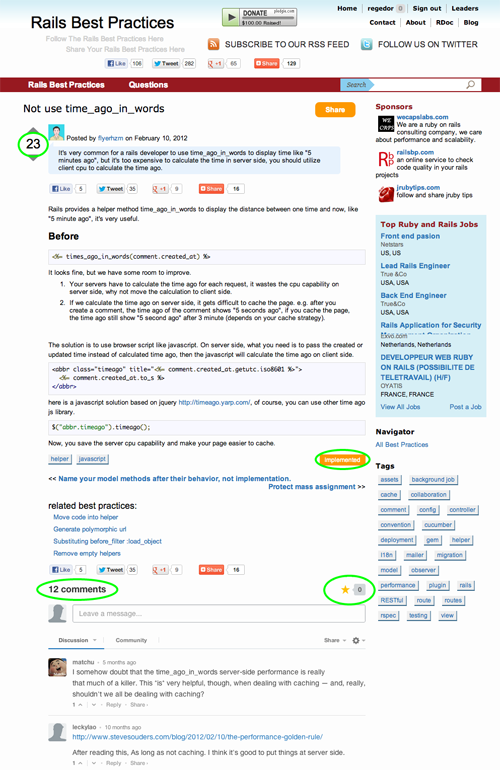
\includegraphics[scale=0.75]{Images/rbp_web}
\end{figure}


After deciding that some \emph{procedure} is a \emph{best practice},
it would be handy to find a way to automatically verify whether 
that practice is being followed by the developers of a given project.
With that in mind, an open source ruby 
\textsf{gem}\footnote{
  Ruby Libraries are called gems. Ruby gems can be easily managed using rubygems 
  (rubygems is for Ruby as aptitude is for Debian or cpan for perl).
}, 
called rails\_best\_practices, was created (by the authors of Rails best practices web site) 
based on the best practices with the most votes. 
After installing the gem, one can run it on any Rails project
and it will automatically produce a report that shows where
in the source code a project is failing to obey to consensual best practices.
It is important to notice that the rails\_best\_practices gem does not indicate if a project is following best practices;
it does the opposite and shows where the project is failing.

At the moment of writing, this gem can check for 33 different best practices from more than 70 described in the web site.
One can read more details about these 33 best practices in Appendix~\ref{app:rails_best_practices}.

During the studies carried out during this thesis, 
we end up forking this project as a starting point for the creation of global best practices metric.
We also did a few commits to this gem source code, now in the official version, to improve it and correct some bugs. 

All the source code is open source and can be found at GitHub (\url{http://www.github.net/regedor}).
Everybody is welcome to contribute to this project by writing more best practices failure detectors,
forking, correcting bugs, or improving it in any way.



